% !TEX program  = xelatex
\documentclass[a4paper]{article}
\usepackage{amsmath}
\usepackage{amssymb}
\usepackage{enumerate}
\usepackage{amstext}
\usepackage{ctex}
%\usepackage{braket}
\usepackage[european]{circuitikz}
\usepackage{multirow}
\usepackage{graphicx}
\usepackage{subfig}
\usepackage{float}
\usepackage{url}
%\usepackage[table,xcdraw]{xcolor}
\usepackage{colortbl}
\usepackage{geometry}
\geometry{left=2.5cm,right=2.5cm,bottom=2.5cm,top=2.5cm}

\title{模电实验报告10:波形变换电路实验}
\author{xy\quad 学号\quad 匡亚明学院}
\date{2019年2月29日}
\begin{document}
\maketitle
\bibliographystyle{unsrt}
%--------main-body------------

\section{实验目的}
\begin{enumerate}
\item 学习使用运放组成精密全波整流电路、电压-频率转换电路。
\end{enumerate}

\section{实验仪器}
示波器、信号发生器、交流毫伏表、数字万用表.

\section{预习内容}
\begin{enumerate}
\item 分析电路图, 定性绘制本实验所用电路的输出波形
\end{enumerate}

\section{实验内容}
\subsection{精密全波整流电路}
\subsubsection{原理}
若直接用二极管整流, 由于普通二极管内限电压为零点几伏, 所以只能用于大信号整流。若要求检波器件的内限电压尽可能地小, 例如1mV, 则可利用运放和二极管可构成这样的检波器件, 如图(\ref{fig1}-(1)), 即等效理想检波二极管, 如图(\ref{fig1}-(2))。

\begin{figure}[!h]
    \qquad
    \subfloat{
    \begin{minipage}[!h]{0.4\textwidth}
        \centering
        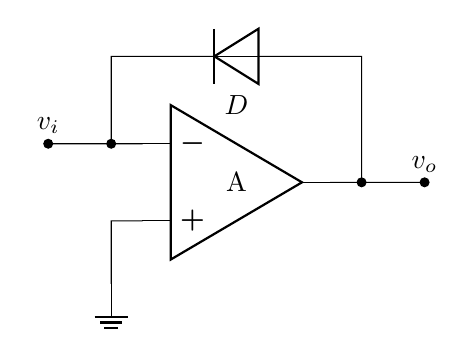
\begin{tikzpicture}[x = 0.8cm, y = 1.6cm]
            \draw (0,0) node[op amp](AMP){} node{A};
            \draw let \p1 = (AMP.-), \p2 = (AMP.+), \p3 = (AMP.out) in
            (AMP.out) -- ++(0.5,0) node[circ](N1){} -- ++(0,1) to [D-, l=$D$] ($(\x1,\y3)+(-0.5,1)$) -- ($(\x1,\y1)+(-0.5,0)$) node[circ](N2){} -- (AMP.-)
            (N2) -- ++(-1,0) node[circ]{} node[anchor = south]{$v_i$}
            (N1) -- ++(1,0) node[circ]{} node[anchor = south]{$v_o$}
            (AMP.+) -- ++(-0.5,0) -- ++(0,-0.5) node[ground]{};
            \end{tikzpicture}
    \caption*{(1)}\label{fig1-1}
    \end{minipage}
    }\qquad\qquad
    \subfloat{
    \begin{minipage}[!h]{0.4\textwidth}
        \centering
        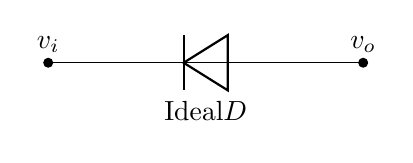
\begin{tikzpicture}[x = 4cm, y = 2cm]
            \draw (0,0) node[anchor = south]{$v_o$} to [D-, l=$\text{Ideal}D$, *-*] ++(-1,0) node[anchor = south]{$v_i$};
            \end{tikzpicture}
    \caption*{(2)}\label{fig1-2}
    \end{minipage}
    }
    \caption{理想检波二极管}\label{fig1}
\end{figure}

在图(\ref{fig1}-(1))中, 若运放输入$V_i$为很小的正电压, 由于运放的开环增益很大, 运放输出$V_o$将为很大的负电压, D1截止;若运放输入$V_i$为很小的负电压, 由于运放的开环增益很大, 运放输出$V_o$将趋向于很大的正电压, D1导通, D1导通后有$V_o$≈$V_i$。可见, 图(\ref{fig1}-(1))等效为一个理想检波二极管。

图(\ref{fig2})就是利用这样的等效理想检波二极管组成的精密全波整流电路。以输入为正弦波为例, 介绍其工作原理。

\begin{figure}[!h]
\centering
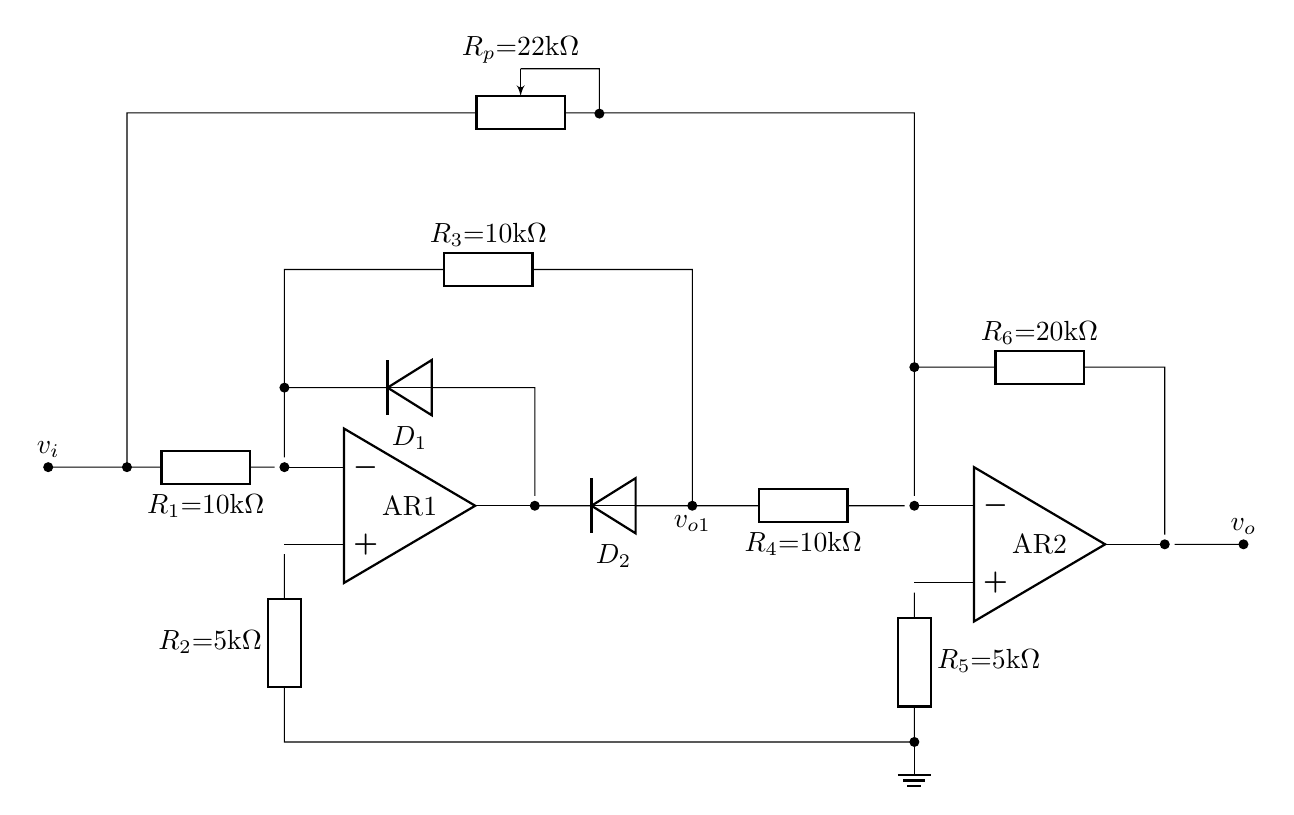
\begin{tikzpicture}[x = 2cm, y = 1.5cm]
    \draw (0,0) node[op amp](AMP){} node{AR1}
    (AMP.-) -- ++(-0.2,0) node(N1){}
    (AMP.+) -- ++(-0.2,0) node(N2){}
    (AMP.out) -- ++(0.2,0) node(N3){};
    \draw let \p1 = (N2) in ($(4,\y1)$) node[op amp](AMP){} node{AR2}
    (AMP.-) -- ++(-0.2,0) node(N4){}
    (AMP.+) -- ++(-0.2,0) node(N5){}
    (AMP.out) -- ++(0.2,0) node(N6){};
    \draw let \p1 = (N1), \p2 = (N2), \p3 = (N3), \p4 = (N4), \p5 = (N5), \p6 = (N6) in
    (N3) to [short, *-] ++(0,1) to [D-, l= $D_1$] ($(\x1,\y3)+(0,1)$) node[circ](T1){} -- ++(0,1) to [R, l= $R_3{=}10\text{k}\Omega$] ($(\x3,\y3)+(1,2)$) -- ++(0,-2) node[circ](VO1){} node[anchor = north]{$v_{o1}$} to [D-, l= $D_2$] ++(-1,0)
    (T1) -- (N1) node[circ]{} to [R, l= $R_1{=}10\text{k}\Omega$] ++(-1,0) node[circ](VI){} -- ++(0,3) to [pR, l= $R_p{=}22\text{k}\Omega$, n = PR] ($(\x4,\y1)+(0,3)$) -- (N4) node[circ]{} to [R, l= $R_4{=}10\text{k}\Omega$] (VO1)
    (PR.wiper) -- ++(0.5,0) -- ++(0,-0.38) node[circ]{};
    \draw let \p1 = (N1), \p2 = (N2), \p3 = (N3), \p4 = (N4), \p5 = (N5), \p6 = (N6) in
    (N6) node[circ]{} to [short] ++(0,1.5) to [R, l_= $R_6{=}20\text{k}\Omega$] ($(\x4,\y6)+(0,1.5)$) node[circ]{};
    \draw let \p1 = (N1), \p2 = (N2), \p3 = (N3), \p4 = (N4), \p5 = (N5), \p6 = (N6) in
    (N6) to [short] ++(0.5,0) node[circ]{} node[anchor = south]{$v_o$}
    (VI) -- ++(-0.5,0) node[circ]{} node[anchor = south]{$v_i$};
    \draw let \p1 = (N1), \p2 = (N2), \p3 = (N3), \p4 = (N4), \p5 = (N5), \p6 = (N6) in
    (N5) to [R, l= $R_5{=}5\text{k}\Omega$] ($(\x5,0)+(0,-2)$) node[ground]{} node[circ]{} -- ($(\x2,0)+(0,-2)$) to [R, l= $R_2{=}5\text{k}\Omega$] (N2);
    \end{tikzpicture}
    \caption{精密全波整流电路}\label{fig2}    
\end{figure}

在正半周期, $V_i$为正, 运放AR1的反相输入端电压为0$^{+}$, 输出趋向于很大的负电压, 二极管D1截止。这里先假设D2导通。那么, 由$R_1$、$R_2$、$R_3$、AR1、D1、D2组成的电路等效为放大倍数为$-$1的放大器, $V_{o1}$输出的波形如图(\ref{fig3}-(2))。当运放AR1的反相输入端电压为0$^{+}$时, 输出趋向于很大的负电压, 而输出$V_{o1}$为输入的反相, 为有限的负电压, 所以D2导通, D2导通后, 运放输出端电压为$-V_i$$-V_{D2th}$, 其中$V_{D2th}$为D2导通时的电压降。可见, 先前假设D2导通是正确的。$V_{o1}$再经由$R_4$、$R_5$、$R_6$、AR2组成的放大倍数为$-$2的放大器, 正半周期输入$V_i$经AR1、AR2组成的两级放大器放大, 形成的输出为$V_{o12}$, 如图(\ref{fig3}-(3)), 为幅值为输入的两倍的正半周期正弦波。与此同时, 输入$V_i$经$R_P$(理论上其阻值应为20k$\Omega$)、$R_6$、$R_5$、AR2组成的放大倍数为$-$1的放大器放大, 形成的输出为$V_{o2}$, 如图(\ref{fig3}-(4))。输入为正半周期时的输出$V_o$为$V_{o12}$与$V_{o2}$的线性迭加, 如图(\ref{fig3}-(5))。显然, 输出波形与输入波形是完全相同的。

\begin{figure}[!h]
\centering
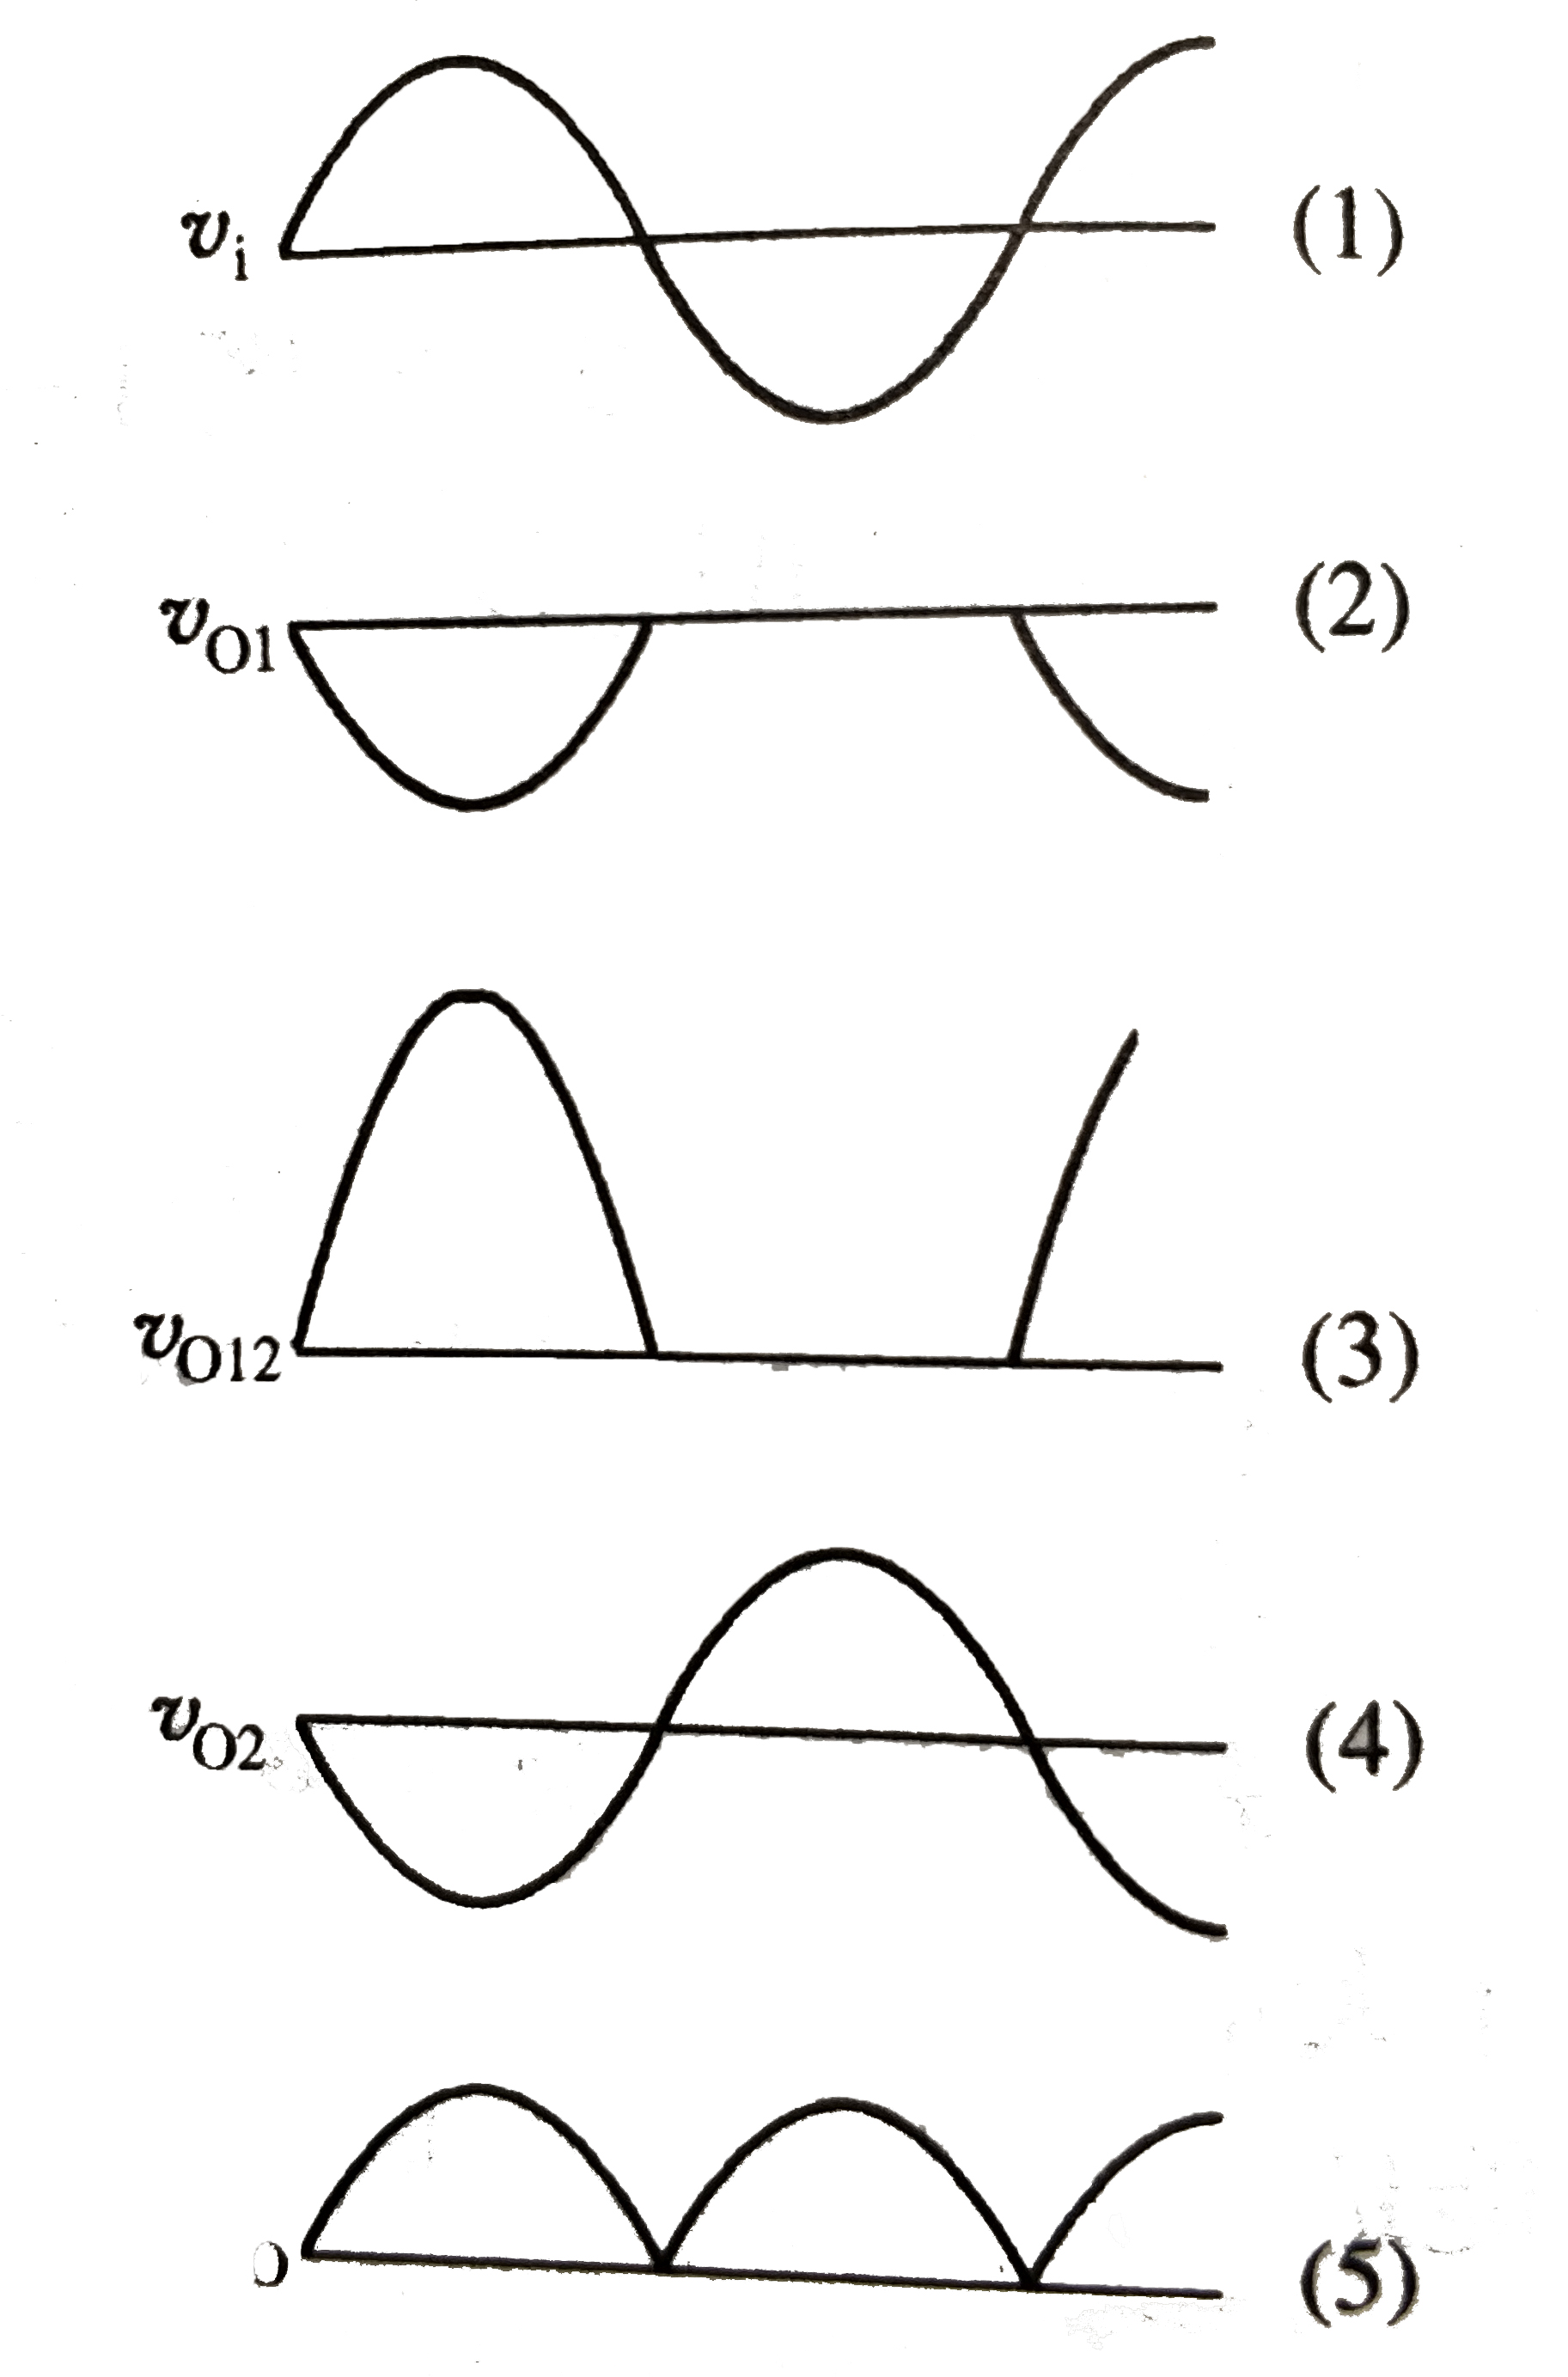
\includegraphics[width=8cm]{fig/fig3.jpg}\\
\caption{图(\ref{fig2})电路各点输出波形分析}\label{fig3}
\end{figure}

在负半周期, $V_i$为负, 运放AR1的反相输入端电压为0$^{-}$, 输出趋向于很大的正电压, 二极管D1导通。这里先假设D2截止。那么, 运放AR1输出端开路。由于AR1的反相输入端电压0$^{-}$, AR2反相输入端电压为0, 所以没有电流流过$R_3$, $V_{o1}$为0, 如图(\ref{fig3}-(2))。当运放AR1的反相输入端电压为0$^{-}$时, 输出趋向于很大的正电压, 而输出$V_{o1}$为0, 可见, 先前假设D2截止是正确的。$V_{o1}$再经由$R_4$、$R_5$、$R_6$、AR2组成的放大器, 输出$V_{o12}$仍为0, 如图(\ref{fig3}-(3))。与此同时, 输入$V_i$经$R_P$(理论上其阻值应为20k$\Omega$)、$R_6$、$R_5$、AR2组成的放大倍数为$-$1的放大器放大, 形成的输出为$V_{o2}$, 如图(\ref{fig3}-(4))。输入为负半周期时的输出$V_o$为$V_{o12}$与$V_{o2}$的线性迭加, 如图(\ref{fig3}-(5))。显然, 输出波形与输入波形是完全相同的。

可见, 在图(\ref{fig2})所示电路中, 若运放为理想运放, $R_P$=$R_6$=2$R_1$, $R_1$=$R_3$=$R_4$, 则输出是对输入的全波整流, 如图(\ref{fig3}-(5))。由于实际元件数值并不等于标称值, 所以实验电路中设置了电位器, 用于调整。由于本实验使用的信号源最小输出是峰值为50mV的正弦电压, 当输入为峰值为50mV的正弦电压时, 实验电路输出应与图(\ref{fig3}-(5))基本相同。

\subsubsection{内容}
\begin{enumerate}
\item 取输入$V_i$有效值为1V、f=1kHz的正弦波。调整$R_P$, 观察输出波形, 使其相邻的峰值尽可能相等。
\item 保持输入信号频率不变, 取输入$V_i$峰值为50mV的正弦波。观察输出波形, 与(1)的输出波形做比较, 试分析造成两者波形差异的原因。
\end{enumerate}
\subsection{电压-频率转换电路}
\subsubsection{原理}
电路如图(\ref{fig4})。这是一个简易的低频压控振荡器。输入为直流电压, 输出为基频频率随输入直流电压变化而变化的锯齿波。

\begin{figure}[!h]
\centering
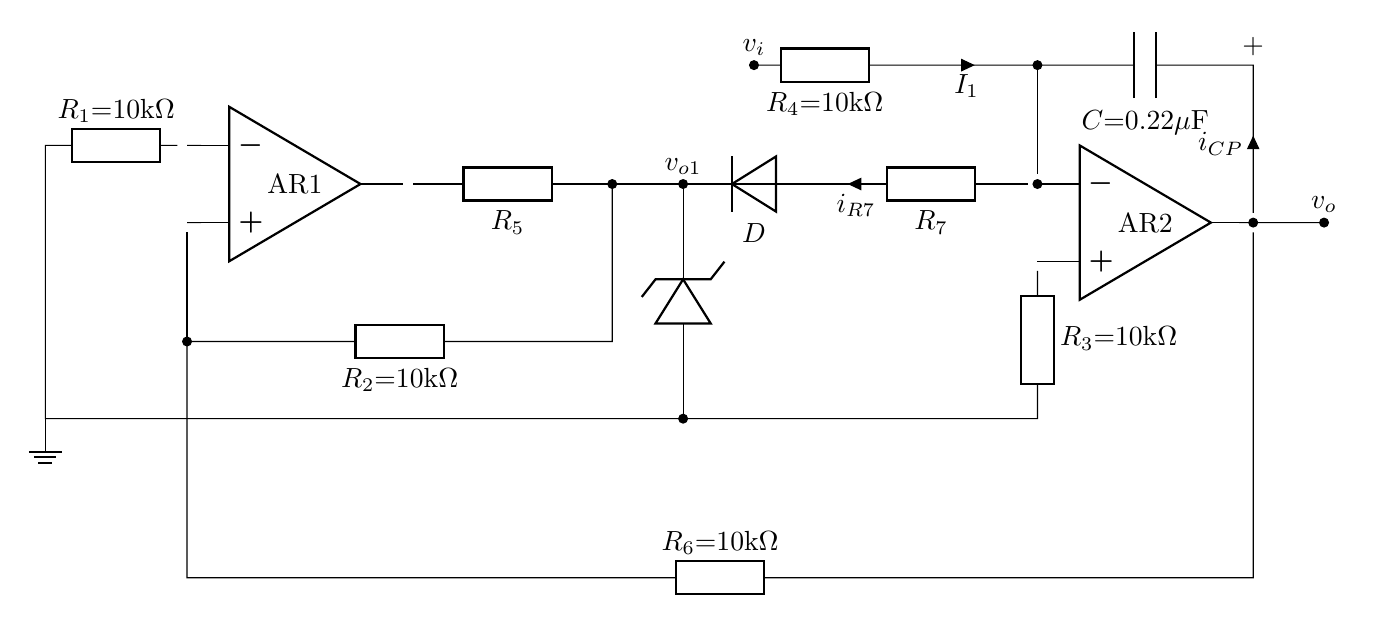
\begin{tikzpicture}[x = 1.8cm, y = 2cm]
    \draw (0,0) node[op amp](AMP1){} node{AR1};
    \draw (AMP1.-) to [short] ++(-0.1,0) node(N1){};
    \draw (AMP1.+) to [short] ++(-0.1,0) node(N2){};
    \draw (AMP1.out) to [short] ++(0.1,0) node(N3){};
    \draw let \p1 = (N2) in ($(6,\y1)$) node[op amp](AMP2){} node{AR2};
    \draw (AMP2.-) to [short] ++(-0.1,0) node(N4){};
    \draw (AMP2.+) to [short] ++(-0.1,0) node(N5){};
    \draw (AMP2.out) to [short] ++(0.1,0) node(N6){};
    \draw let \p1 = (N1), \p2 = (N2), \p3 = (N3), \p4 = (N4), \p5 = (N5), \p6 = (N6), \p7 = (AMP1.+) in
    (N4) to [R, l=$R_7$, i=$i_{R7}$] ++(-1.5,0) to [D-, l=$D$] ++(-1,0) node[circ](VO1){} node[anchor = south]{$v_{o1}$} -- ++(-0.5,0) node[circ](T1){} to [R, l=$R_5$] (N3);
    
    \draw let \p1 = (N1), \p2 = (N2), \p3 = (N3), \p4 = (N4), \p5 = (N5), \p6 = (N6), \p7 = (AMP1.+) in
    (T1) -- ++(0,-1) to [R, l=$R_2{=}10\text{k}\Omega$] ($(\x1,\y3)+(0,-1)$) node[circ](T2){} -- ++(0,-1.5) to [R, l=$R_6{=}10\text{k}\Omega$] ($(\x6,\y3)+(0,-2.5)$) to [short] (N6) node[circ](VO){} to [short, i=$i_{CP}$] ++(0,1) node[anchor = south]{+} to [C, l=$C{=}0.22\mu\text{F}$] ($(\x4,\y6)+(0,1)$) node[circ](T3){} to [short, i<=$I_1$] ++(-1,0) to [R, l=$R_4{=}10\text{k}\Omega$] ++(-1,0) node[circ]{} node[anchor = south]{$v_i$};
    \draw let \p1 = (VO1), \p2 = (N1), \p3 = (N5) in
    (N5) to [R, l=$R_3{=}10\text{k}\Omega$] ++(0,-1) -- ($(\x1,\y3)+(0,-1)$) node[circ](T4){} -- ($(\x2,\y3)+(-1,-1)$) node[ground]{} -- ($(\x2,\y2)+(-1,0)$) to [R, l=$R_1{=}10\text{k}\Omega$] (N1);
    
    \draw let \p1 = (N1), \p2 = (N2), \p3 = (N3), \p4 = (N4), \p5 = (N5), \p6 = (N6), \p7 = (AMP1.+) in
    (T2) to [short] (N2);
    \draw (VO) to [short] ++(0.5,0) node[circ]{} node[anchor = south]{$v_o$};
    \draw (T3) to [short, -*] (N4);
    \draw (T4) to [empty ZZener diode] (VO1)
    
    
    ;
    \end{tikzpicture}
    \caption{低频压控振荡器}\label{fig4}    
\end{figure}

在稳态。设在$V_{o1}$=$V_z$ 、$V_o$=$-V_z$时刻, 运放AR1正相输入端电压过0, 趋向负, $V_{o1}$翻转, 由$V_z$变为$-V_z$。如图(\ref{fig5}), 向电容正向充电的电流$i_{CP}$为
\begin{equation}
i_{CP} = i_{R_7} - i_i = \cfrac{V_z - V_{Dth}}{R_7} - \cfrac{V_i}{R_4}\label{eq1}
\end{equation}
其中, $V_{Dth}$为二极管的导通电压。向电容正向充电使输出电压$V_o$上升, 当输出电压上升到$V_o$=$V_z$时, AR1正相输入端的电压再次过0, 但趋向于正, $V_{o1}$再次翻转, 由$-V_z$变为$V_z$。记此过程持续的时间为T1, 在此过程中, 输出电压的变化量为
\begin{equation}
V_o = \cfrac{1}{C}\int^{T_1}_{0}\left(\cfrac{V_z - V_{Dth}}{R_7} - \cfrac{V_i}{R_4}\right)\text{d}t = \left(\cfrac{V_z - V_{Dth}}{R_7C} - \cfrac{V_i}{R_4C}\right)T_1 = 2V_z\label{eq2}
\end{equation}

\begin{figure}[!h]
\centering
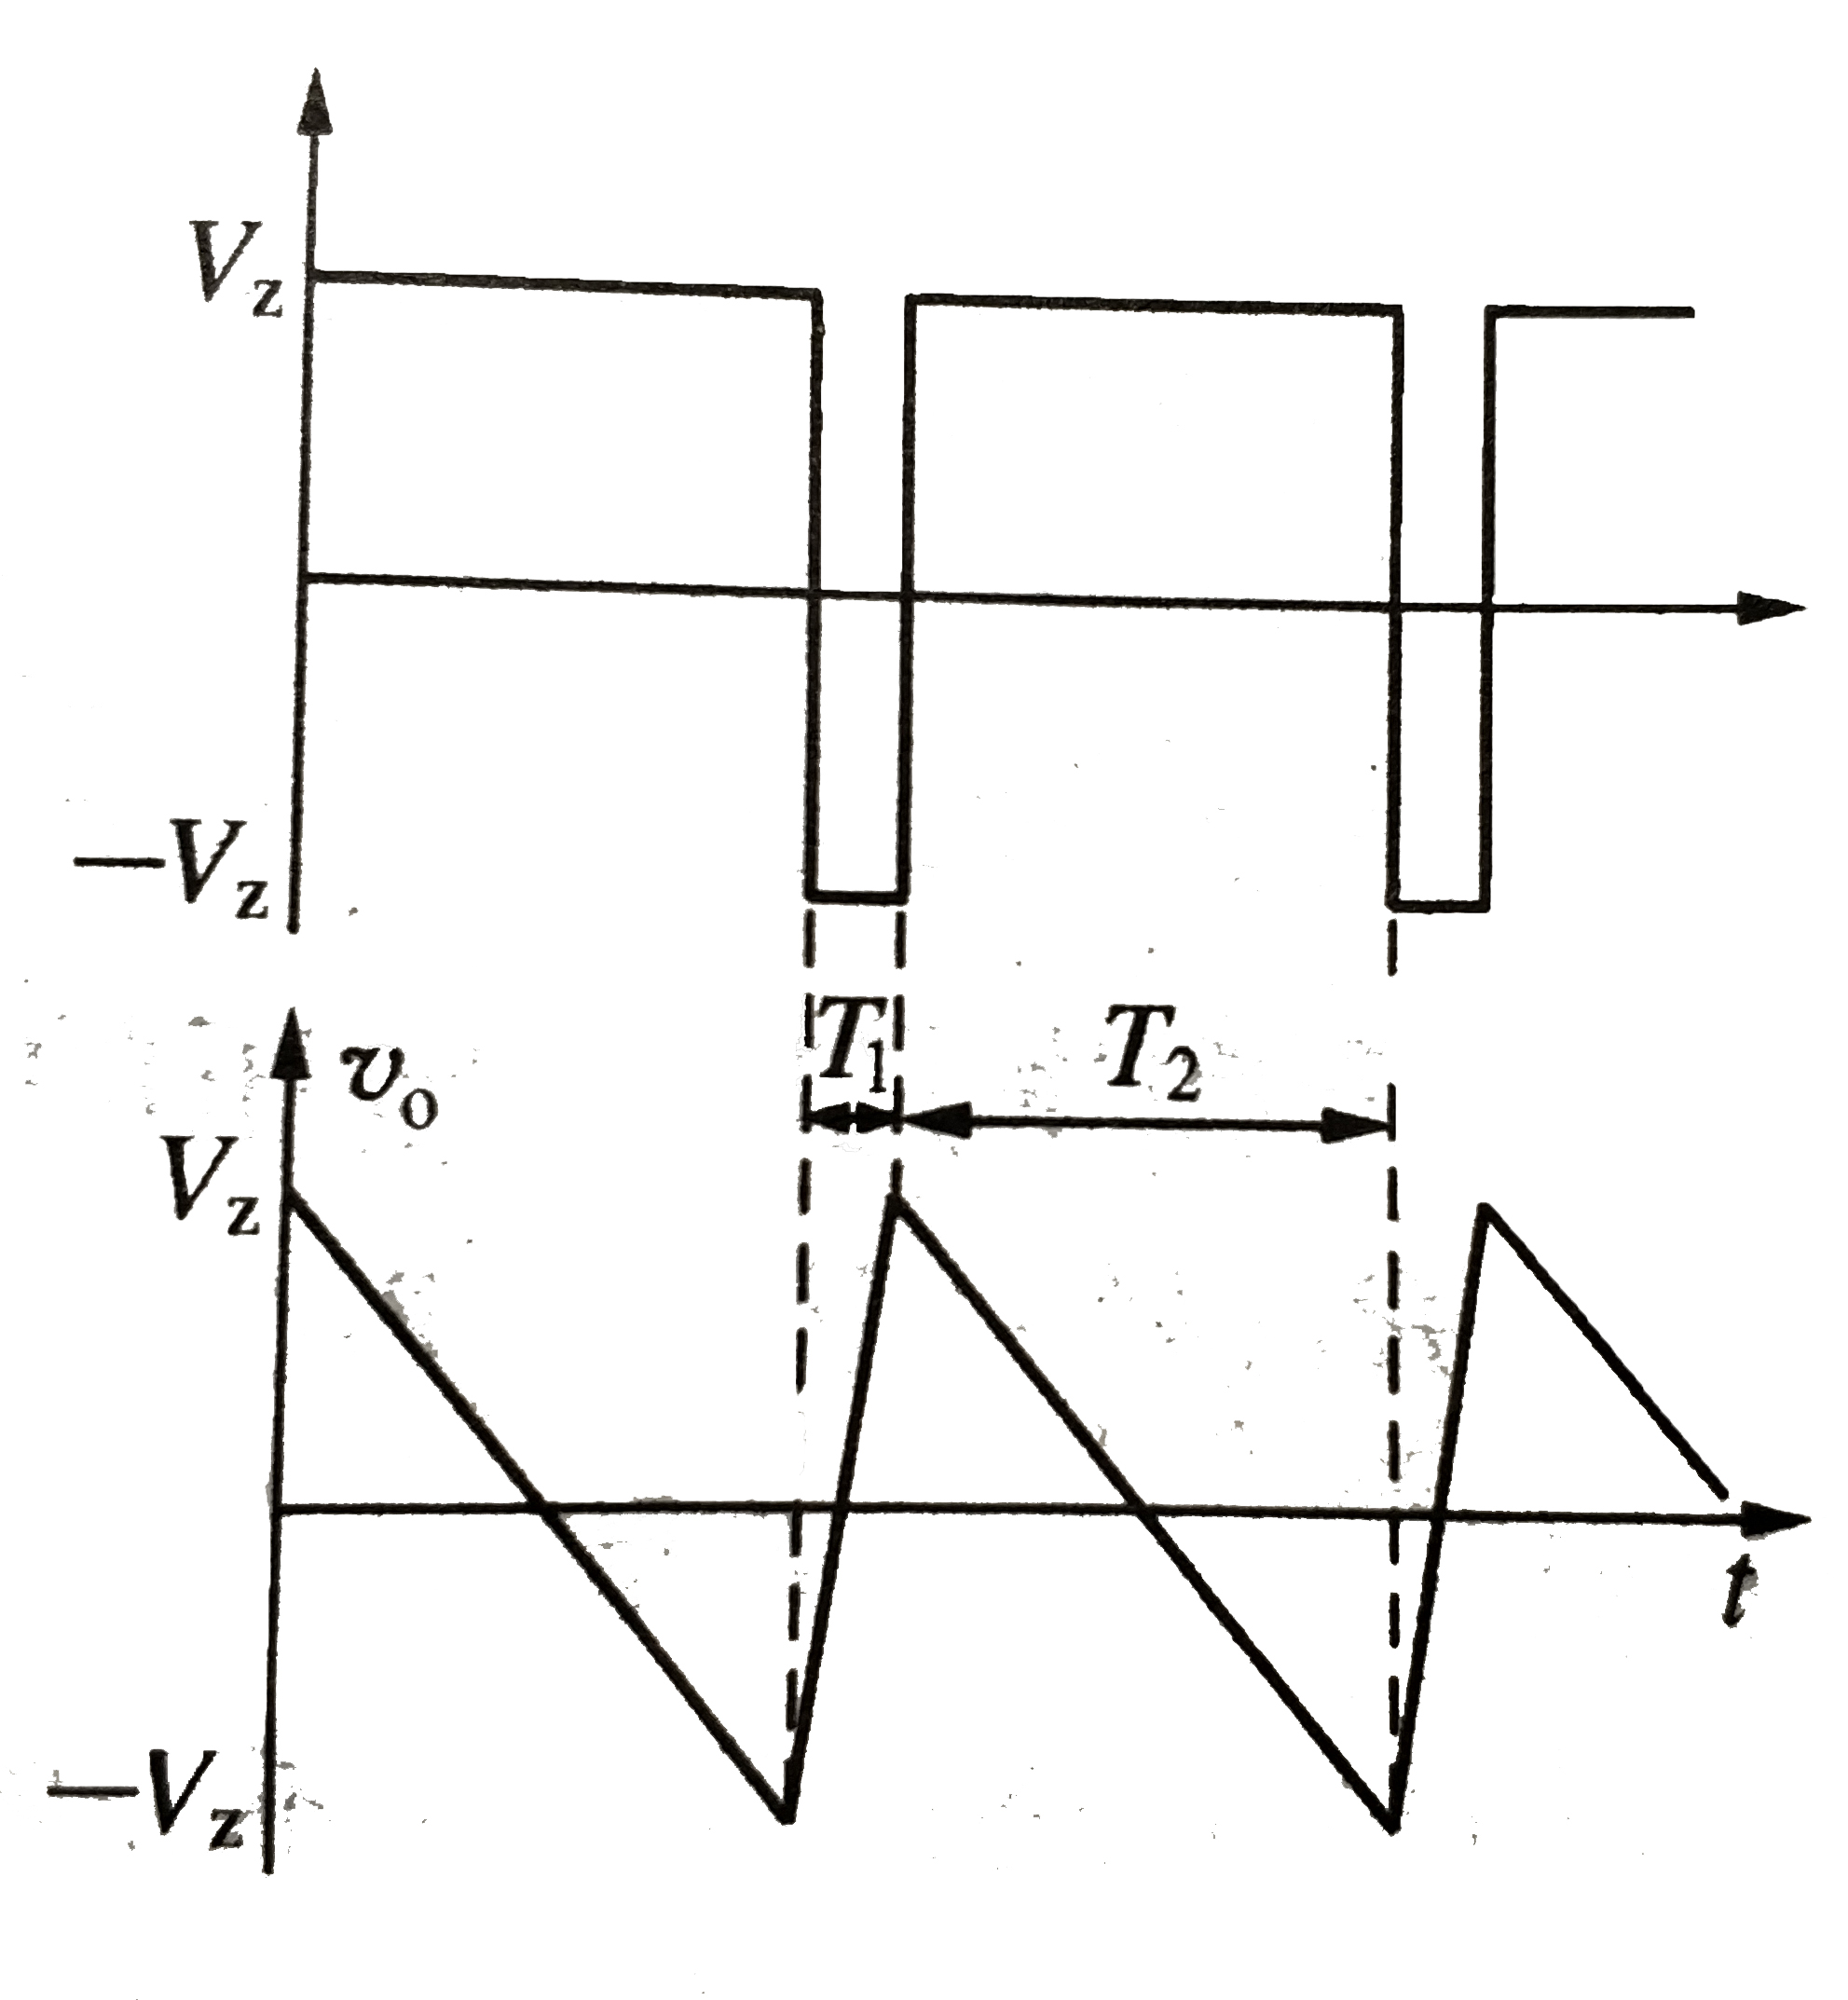
\includegraphics[width=8cm]{fig/fig5.jpg}\\
\caption{图(\ref{fig4})所示电路的输出波形}\label{fig5}
\end{figure}
    
从中可解出
\begin{equation}
T_1 = \cfrac{2V_z}{\cfrac{V_z - V_{Dth}}{R_7C} - \cfrac{V_i}{R_4C}}\label{eq3}
\end{equation}
紧接着, 由于$V_{o1}$=$V_z$, AR2反相输入端为“虚地”, 这使得二极管D截止, 只有$V_i$ 向电容反向充电, 充电电流为
\begin{equation}
i_{CN} = -\cfrac{V_i}{R_4}\label{eq4}
\end{equation}
向电容反向充电使输出电压$V_o$下降, 当输出电压下降到$V_o$=$-V_z$时, AR1正相输入端的电压过0, 趋向于负, $V_{o1}$翻转, 由$V_z$变为$-V_z$。记此过程持续的时间为$T_2$, 在此过程中, 输出电压的变化量为
\begin{equation}
V_o = -\cfrac{1}{C}\int^{T_2}_{0}i_{CN}\text{d}t = -\cfrac{1}{C}\int^{T_2}_{0}\cfrac{V_i}{R_4}\text{d}t = -\cfrac{V_i}{R_4C}T_2 = -2V\label{eq5}
\end{equation}
从中可解出
\begin{equation}
T_2 = 2R_4C\cfrac{V_z}{V_i}\label{eq6}
\end{equation}
输出$V_o$的波形如图(\ref{fig5}), 为锯齿波。其基频频率为
\begin{equation}
f = \cfrac{1}{T_1+T_2} = \cfrac{(V_z - V_{Dth})R_4V_i - R_7V_i^2}{2(V_z - V_{Dth})V_zR_4^2C} = \cfrac{V_i}{2R_4CV_z} - \cfrac{R_7V_i^2}{2(V_z - V_{Dth})V_zR_4^2C}\label{eq7}
\end{equation}
可见, 基频频率是输入电压的二次函数, 其函数曲线如图(\ref{fig6})。

\begin{figure}[!h]
\centering
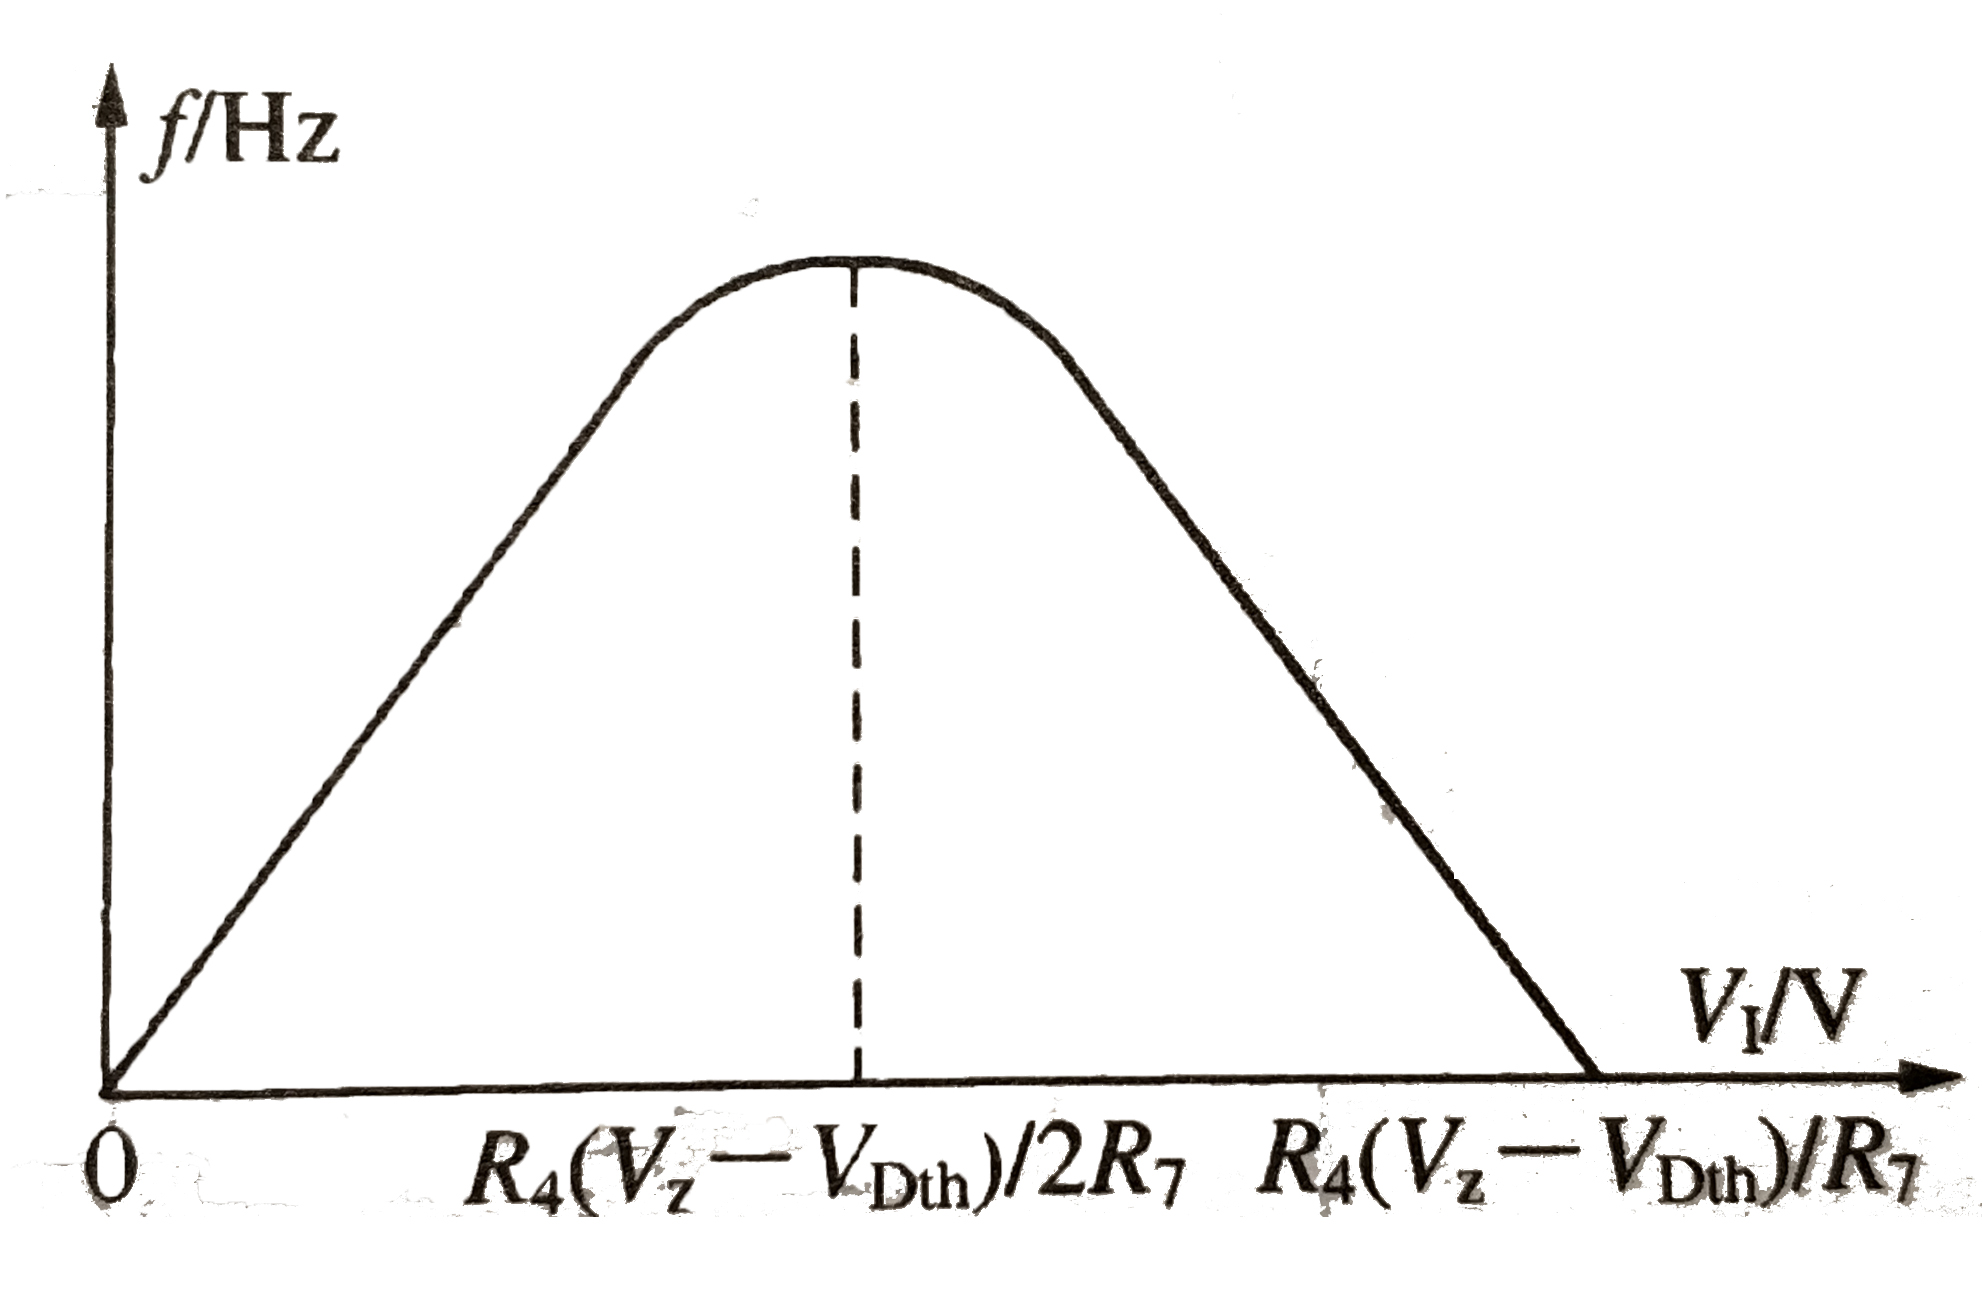
\includegraphics[width=10cm]{fig/fig6.jpg}\\
\caption{输出波形频率-输入直流电压特性曲线}\label{fig6}    
\end{figure}

当0<$V_i$<R4($V_z$-$V_{Dth}$)/2$R_7$时, 基频频率随输入电压增加而单调上升。人们通常希望基频频率f是输入电压$V_i$的一次函数, 这就要求(\ref{eq7})式中的$R_7$较小。但就电路而言, $R_7$不能很小, 因为AR2反相输入端电位近似为0, $V_{o1}$为低时约为-6V, 若此电压全部加在二极管D上, 二极管正向导通电压约为零点几伏, 则电路无法正常工作。建议在实验中$R_7$取1k$\Omega$, 或取1k$\Omega$电位器, 在实验中再调整。若再设$V_{Dth}$=0.7V, 则(\ref{eq7})式可写为
\begin{equation}
f \approx 37.88V_i - 0.7147V_i^2\label{eq8}
\end{equation}
若输入电压较小, 也可使频率f近似为输入电压$V_i$的一次函数。由(\ref{eq8})式可知, 当$V_i$为26.5V时, f取最大值。若实验中取0$<V_i<$5V, 由图(\ref{fig6})可见, f近似为输入电压$V_i$的一次函数。

在本实验电路中, 当$V_{o1}$=$-V_z$时, 流经$R_7$的电流将灌入运放AR1;同时, 为稳定$V_{o1}$=$-V_z$=-6V, 由“地”流经稳压二极管的电流也将灌入运放AR1。若限流电阻$R_5$过大, $V_{o1}$将上升, 这在示波器可清楚地看到,  $V_{o1}$波形上下幅值严重不对称, 正向幅值大, 负向幅值小。而(\ref{eq7})式是在图(\ref{fig5})所示的$V_{o1}$波形上下对称时推导出来的, 所以测量到的频率值将较大地大于用(\ref{eq8})式估算的频率值。这时应减小$R_5$, 使$V_{o1}$波形的反相幅值略小于正相幅值即可, R5不宜过小, 建议取1k$\Omega$<R5<3k$\Omega$。
\subsubsection{内容}
\begin{enumerate}
\item 取输入电压$V_i$=1V, 选取适当的$R_5$, 使$V_{o1}$波形上下幅值近似相等。选取$R_7$(可取500至1000$\Omega$)。
\item 测量并绘制输出波形频率-输入直流电压特性曲线, 取输入直流电压V(0.1, 5)V。并与理论估算值相比较。
\end{enumerate}

\section{实验数据}
\subsection{精密全波整流电路}
在此实验中,$R_P$ = 19.8505k$\Omega$。
\subsubsection{$v_{irms}$ = 0.9893V}
\begin{figure}[!h]
\centering
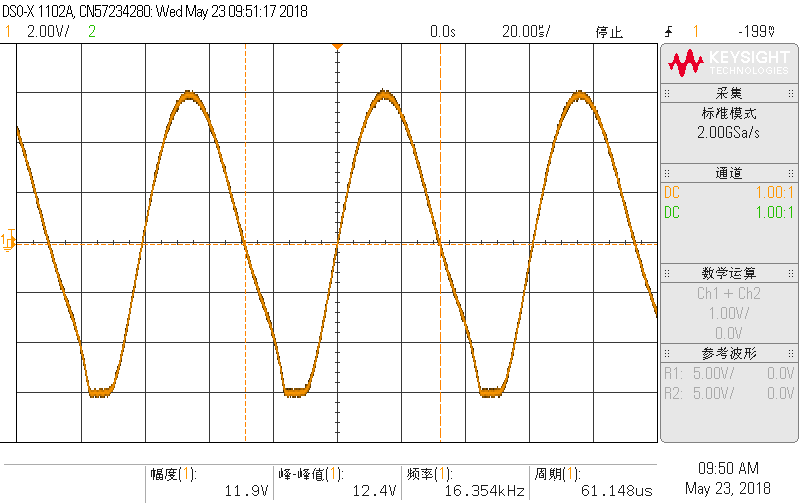
\includegraphics[width=12cm]{../data/scope_1.png}\\
\caption{$v_{irms}$ = 0.9893V时的波形图}\label{datafig1}
\end{figure}
\subsubsection{$v_{ipp}$ = 50mV}
此时$v_{irms}\approx$17.545mV
\begin{figure}[!h]
\centering
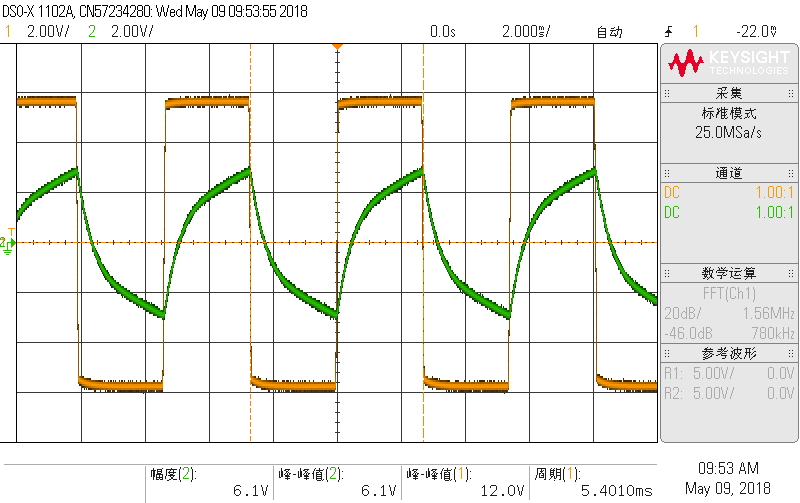
\includegraphics[width=12cm]{../data/scope_2.png}\\
\caption{$v_{ipp}$ = 50mV时的波形图}\label{datafig2}
\end{figure}

\subsection{电压-频率转换电路}
输入信号$V_I$ = 1.0004V,$R_5$ = 5.1k$\Omega$,$R_7$ = 1k$\Omega$。
\begin{figure}[!h]
\centering
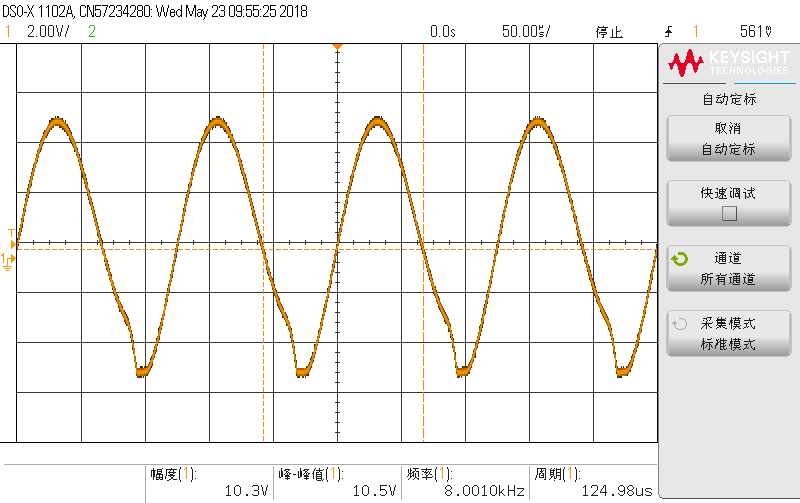
\includegraphics[width=12cm]{../data/scope_3.png}\\
\caption{电压-频率转换电路波形图}\label{datafig3}
\end{figure}

测得的输出信号频率于输入信号电压关系曲线如图(\ref{Vfreq}),可见电压-频率曲线与抛物线符合较好,拟合公式标在图中。
\begin{figure}[!h]
\centering
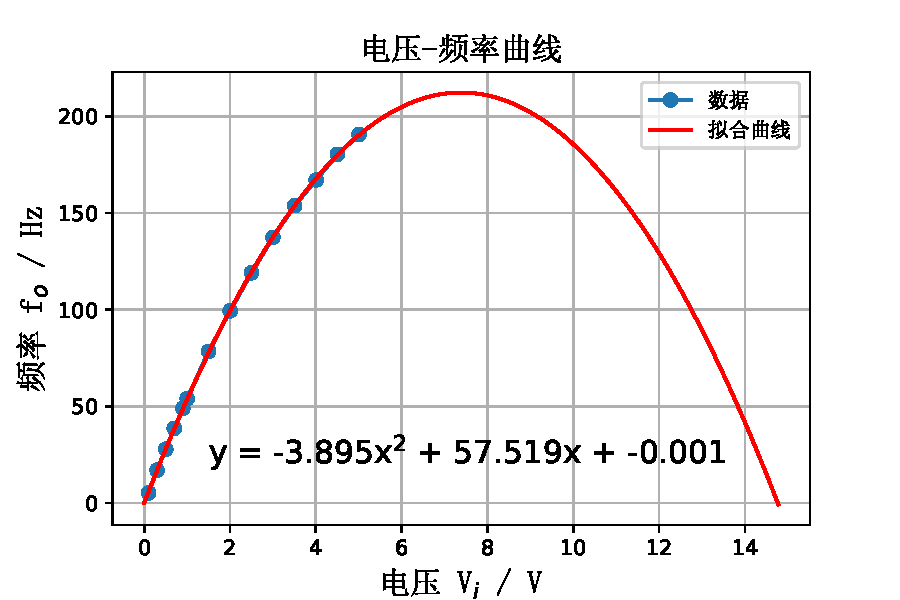
\includegraphics[width=12cm]{fig/Vfreq.pdf}\\
\caption{测得输出频率-输入电压特性曲线}\label{Vfreq}
\end{figure}

\section{实验讨论}
\begin{enumerate}
\item 如图(\ref{datafig2}),精密整流电路在输入信号极小时,输出波形失真严重,且波形不好看,应该是接近了运放的灵敏度的极限。
\end{enumerate}

\section{思考题}
\subsection{若要求输出为整流后的波形的直流分量, 应如何修改图(\ref{fig2})所示电路?当输入$V_i$有效值为1V时, 这个直流分量应为多少伏?}
在输出端接一个电容到地,这样可以滤去输出信号的交流成分。电容的容值可取10mF。
\subsection{若输入为正弦分量加直流分量, 在输出端仅要求反映正弦分量, 应如何修改图(\ref{fig2})所示电路?设f=1kHz, 给出具体的元件参数。}
应该在输入端加一个电容,滤去直流分量而通过交流分量。可以取电容的值为10mF。

\nocite{jiaocai}
%--------bib------------------
\bibliography{ref}
\end{document}